% ----------------------------------------------------------
\chapter{Revisão Bibliográfica}
% ----------------------------------------------------------

Para atingir o objetivo de projetar o \textit{hardware} de um computador de bordo, foi preciso buscar na literatura acadêmica o estado da arte que tange o projeto de OBDHs para satélites de pequeno porte, especialmente para CubeSats.
 
No primeiro tópico, será apresentado um breve estudo sobre a radiação em LEO (\textit{Low Earth Orbit}, órbitas com raio menor que 1000 km, segundo ESA, 2024), para entender os possíveis efeitos em componentes eletrônicos do CubeSat, baseando-se em diferentes autores. Dessa forma, buscaram-se formas de mitigar os efeitos mais conhecidos e verificar como os projetos têm lidado com componentes do tipo \textit{Commercial-Off-The-Shelf} (COTS).% Além disso, também foi dada a fundamentação dos conversores de potência, tipos de memória, microprocessadores e interfaces de comunicação.

Depois disso, serão analisadas diversas placas de computadores de bordo desenvolvidos pela indústria e pela academia, a fim de compreender o estado da arte. Aqui, destacam-se as placas de OBDH dos projetos do FloripaSat-1 e FloripaSat-2, desenvolvidos pelo SpaceLab da UFSC, precursores principais do OBDH a ser desenvolvido nesse trabalho, bem como o Nanomind Z7000, projetado e fabricado pela GomSpace, utilizando um SoC como processador. Um panorama geral será feito, verificando-se principalmente os componentes principais e mais críticos, ou seja, processadores, memórias e outros periféricos.

Por fim, será explicitada a metodologia escolhida para a seleção dos componentes do OBDH projetado, de acordo com o estado da arte e com diretrizes e normas relevantes. Essa explicitação será crucial para que os componentes COTS sejam os melhores possíveis nos quesitos de temperatura e tolerância a falhas.

\section{Radiação em LEO e Componentes COTS}

Estando em solo terrestre, os componentes eletrônicos estão bem protegidos contra a maior parte da radiação incidente do universo, sejam elas raios cósmicos, partículas solares ou \textit{trapped radiation}. No caso dos satélites orbitais, a proteção atmosférica é nula, mesmo para aqueles que operam em LEO. Nesse caso, a radiação pode ser suficientemente significativa para causar a mudança do comportamento eletromagnético dos materiais, causando efeitos como falhas, aquisição ou execução errada de comandos e distorções dos sinais (MAYANBARI, 2011) (LABEL, 2004).  Esses danos são divididos em dois grupos (JUNQUEIRA, 2020): os acumulativos como o TID (\textit{Total Ionizing Dose}), e os SEE (\textit{Single Event Effects}), que indicam o acontecimento de eventos únicos. 

O TID (Figura \ref{fig:tid}), segundo Junqueira (2020), se caracteriza principalmente pela formação de pares elétron-lacuna, onde o primeiro aumenta a condutividade do material e o segundo contribui para oxidação, mudando as características elétricas do componente com o tempo.  Já os SEE (Figura \ref{fig:see}) ocorrem quando um íon atravessa um componente crítico, gerando uma linha de ionização que pode ou não ser destrutiva. 

\begin{figure}[H]
    \centering
    \caption{Esquema representativo do TID.}
    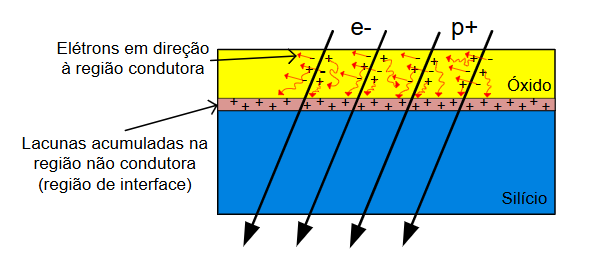
\includegraphics[scale=0.8]{images/tid.png}
    \label{fig:tid}
    \fonte{JUNQUEIRA, 2020.}
\end{figure}

\begin{figure}[H]
    \centering
    \caption{Esquema representativo do SEE.}
    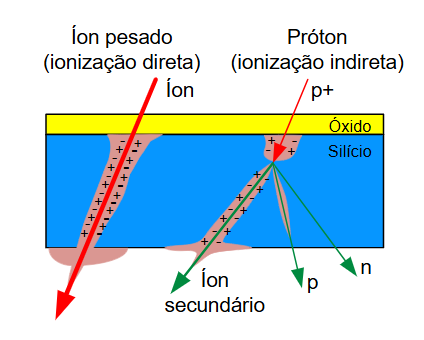
\includegraphics[scale=0.8]{images/see.png}
    \label{fig:see}
    \fonte{JUNQUEIRA, 2020.}
\end{figure}

Especialmente nesse trabalho, o efeito denominado SEL (\textit{Single Event Latch-up}) tem seu destaque. Por ser um tipo de SEE, ocorre após uma partícula carregada atravessar e atingir o substrato do circuito integrado, gerando correntes parasitas que podem ser superiores ao valor máximo suportado pelo componente (JUNQUEIRA, 2020). Proteger os barramentos de alimentação contra esse efeito será crucial para a arquitetura proposta nesse trabalho.

Por esse motivo, quando são escolhidos os componentes críticos para o \textit{hardware} de um \textit{CubeSat}, em sua maioria COTS, deve-se levar em consideração algumas diretrizes principais. Segundo Carmo et al. (2021), o componente escolhido precisa atender os requisitos operacionais, concomitante ao gerenciamento de riscos com mitigações (uso de FRAM, proteção contra \textit{latch-up}, entre outros) e blindagens (uso de \textit{shields} de metal). 

Outro aspecto da seleção de componentes será explorado na seção a seguir, avaliando os OBDHs comerciais e da academia, explorando a característica de herança de voo.

\section{Projetos Anteriores}

\subsection{FloripaSat-1}
% https://ieeexplore.ieee.org/abstract/document/9085277
O FloripaSat-1 (MARCELINO et al., 2020) é uma plataforma \textit{open-source} para nanossatélites, além de ser também o nome do primeiro satélite inteiramente desenvolvido e lançado pelo SpaceLab. O satélite FloripaSat-1 é um CubeSat 1U,  composto de três módulos: um módulo de fornecimento de potência (EPS), um computador de bordo (OBDH) e um módulo de telemetria e comunicação (TTC). Além disso, possuía duas cargas úteis que consistiam de placas com FPGAs. A missão tinha como objetivos a validação do satélite em órbita dos módulos desenvolvidos na UFSC e de um módulo com um FPGA tolerante a radiação.

Seu OBDH foi feito para realização da interface e comunicação entre os módulos e \textit{payloads}. Aqui, destacam-se os sensores presentes: uma \textit{Inertial Measurement Unit} (com giroscópio, magnetômetro e acelerômetro), a interface com os sensores dos painéis solares e as medições de tensão e corrente de entrada do próprio módulo.

Além disso, contava com um microprocessador de 16 bits (MSP430), memórias flash (IS25LP128) e suporte para cartão microSD para armazenamento.

\subsection{FloripaSat-2}
% https://ieeexplore.ieee.org/abstract/document/10078027
O FloripaSat-2 é a segunda geração da plataforma \textit{open-source} desenvolvida pelo SpaceLab, baseando-se no projeto FloripaSat-1 e trazendo melhorias para os três módulos principais (MARCELINO et al., 2024). O diagrama de blocos do CubeSat proposto está disposto na Figura \ref{fig:floripasat2}, onde pode-se verificar as interfaces do OBDH com o restante do módulo.

\begin{figure}[H]
    \centering
    \caption{Diagrama de blocos da plataforma FloripaSat-2.}
    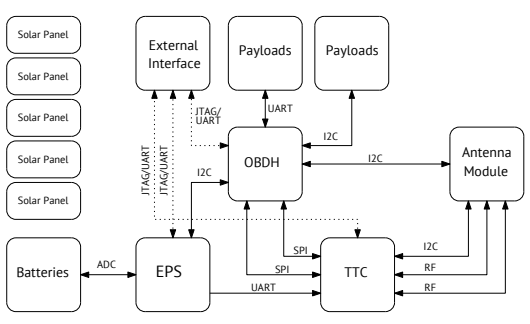
\includegraphics[scale=0.8]{images/floripasat2.png}
    \label{fig:floripasat2}
    \fonte{MARCELINO et al., 2024.}
\end{figure}

Especificamente para o OBDH, foram introduzidas uma memória FRAM (\textit{Ferroelectric Random-Access Memory}) e uma Flash NOR de maior capacidade de armazenamento, o que mostra uma melhoria clara de capacidade e confiabilidade. Outras duas melhorias importantes foram, primeiramente, a adição de um conector para eventualmente conectar uma \textit{daughter board} à placa, e, segundamente, a adição de \textit{buffers} aos barramentos de I2C (\textit{Inter-Integrated Circuit}) entre os módulos. Isso acrescenta flexibilidade e confiabilidade ao OBDH da segunda geração. Esse projeto será utilizado nas missões GOLDS-UFSC, Catarina-A1 e A3 e Aldebaran-1, que ainda não foram lançadas.

\subsection{Projetos Comerciais}

Abaixo se encontram sintetizados os projetos comerciais estudados, para obtenção de noções sobre a arquitetura e componentes usados. Foram verificados principalmente os processadores, as memórias voláteis e não-voláteis, as interfaces de comunicação e outros periféricos (ADCs, RTC, etc.) utilizados. A Tabela \ref{tab:Tab_Rev} mostra a pesquisa realizada sobre o estado da arte, em conjunto com os dados de George e Wilson (2018), sintetizados na Tabela \ref{tab:Tab_Missoes}.

\begin{table}[htb]
    \centering
	\ABNTEXfontereduzida
	\caption{\label{tab:Tab_Rev}Comparação entre os principais modelos comerciais de OBDH disponíveis atualmente no mercado.}
	%\begin{tabular}{@{}p{2cm}p{2cm}p{2cm}p{2cm}p{2cm}p{2cm}p{3cm}@{}}
    \begin{tabular}{@{}p{2cm}p{2.6cm}p{2cm}p{2cm}p{2.2cm}p{2.6cm}@{}}
		\toprule
		\textbf{Fabricante} & \textbf{Nome do Produto} & \textbf{Processador} & \textbf{Memórias} & \textbf{Periféricos} & \textbf{Interfaces de comunicação} \\ 
        \midrule
        GomSpace & NanoMind A3200 & AT32UC3C & Flash, SDRAM, FRAM & Giroscópio, Magnetômetro, Transceivers, Sensores de temperatura & CAN, I2C, SPI, JTAG, USART \\%https://gomspace.com/UserFiles/Subsystems/datasheet/gs-ds-nanomind-a3200_1006901-117.pdf
        
        \midrule
        GomSpace & NanoMind HPMK3 & Zynq 7030 & Flash, eMMC, DDR3 & Watchdog, Sensores de temperatura, VCO, Sensores de tensão e corrente & CAN, USART, USB, I2C, JTAG, LVDS, SpaceWire \\ %https://gomspace.com/UserFiles/Subsystems/datasheet/gs-ds-NanoMind_HP_MK3.pdf

        \midrule
        ISIS Space & ISIS On Board Computer & Atmel & Flash, SDRAM, FRAM, Cartões SD & Sensores de temperatura, Sensores de tensão e corrente, RTC, ADC & USART, USB, I2C, JTAG, PWM \\ %https://www.isispace.nl/product/on-board-computer/

        \midrule
        Nano Avionics & SatBus 3C2 & Não informado & Flash, FRAM, Cartões SD & Giroscópio, Magnetômetro, Rádio UHF, ADC & CAN, SPI, I2C, USART, PWM, USB \\ %https://nanoavionics.com/cubesat-components/cubesat-on-board-computer-main-bus-unit-satbus-3c2/

        \midrule
        AAC Clyde Space & Kryten-M3 & Smart Fusion 2 SoC & MRAM, eNVM & RTC, Sensores de tensão e corrente & CAN, SPI, I2C, USART, RS422, LVDS \\ %https://www.aac-clyde.space/what-we-do/space-products-components/command-data-handling/kryten-m3       


		
        \\ \bottomrule
	\end{tabular}
	\fonte{Elaboração própria.}
\end{table}

\begin{table}[H]
	\ABNTEXfontereduzida
	\caption{\label{tab:Tab_Missoes}Síntese da tabela apresentada por George e Wilson (2018).}
	%\begin{tabular}{@{}p{2cm}p{2cm}p{2cm}p{2cm}p{2cm}p{2cm}p{3cm}@{}}
    \centering
    \begin{tabular}{@{} >{\centering}p{3.5cm} >{\centering}p{3.5cm} >{\centering}p{3.5cm} @{}}
    
		\toprule
		\textbf{Fabricante} & \textbf{Processadores} & \textbf{Missões por Fabricante} \tabularnewline 
        \midrule
        Xilinx & Zynq 7020, Zynq 7030, Zynq 7045, Ultrascale+, etc. & 24 \tabularnewline
        
        \midrule
        Atmel + Microchip & ATmega329P, AT91SAM9G20, PIC24F, etc. & 22 \tabularnewline 

        \midrule
        Texas Instruments & MSP430, OMAP3530, Sitara AM3703, etc. & 15 \tabularnewline 

        \midrule
        Cobham Gaisler & GR712RC, UT699, LEON3FT & 8 \tabularnewline
        
        \bottomrule
	\end{tabular}
	\fonte{Elaboração própria com base em George e Wilson, 2018, página 463.}
\end{table}

Comparando ambas tabelas, é possível verificar que a maioria dos processadores apresentados, no contexto explorado por (GEORGE E WILSON,  2018), são de duas fabricantes: Xilinx (especialmente \textit{chips} da família Zynq 7000) e Microchip (incluindo Atmel). Além disso, a maior parte dos projetos comerciais vistos apresentam memórias FRAM, que possuem um número máximo de ciclos de leitura e escrita muito elevada, além de memórias Flash. Outro destaque foi a presença de sensores de tensão e corrente, bem como magnetômetros e giroscópios.

Além disso, projetos como o OBDH Nanomind Z7000 (GomSpace Nanomind Z7000 Datasheet, 2019) demonstraram sua efetividade em diversas missões, como FSSCAT (CAMPS et al., 2018), ORCA (BARLES et al., 2022) e CubeMAP (WEIDMANN et al., 2020), o que mostra a confiabilidade e herança de voo de \textit{hardwares} contendo SoCs (\textit{System-on-a-Chip}) da família Zynq 7000. Na Figura \ref{fig:nanomind}, podemos verificar o diagrama de blocos do anteriormente citado Nanomind Z7000.

\begin{figure}[H]
    \centering
    \caption{Diagrama de blocos do OBDH Nanomind Z7000.}
    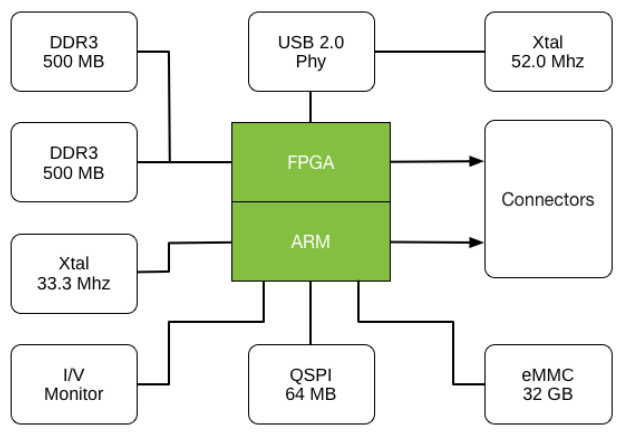
\includegraphics[scale=0.8]{images/nanomind z7000.png}
    \label{fig:nanomind}
    \fonte{GomSpace Nanomind Z7000 Datasheet, 2019.}
\end{figure}

\subsection{Projetos Acadêmicos}

Outro ponto são os OBDHs propostos em publicações acadêmicas. Serão estudados quatro casos de design de OBDH, ainda no contexto de nanossatélites. 

No primeiro caso, o OBDH foi feito para ser compacto e reconfigurável, como o projeto proposto nesse trabalho. O sistema foi pensado para conter um processador, SDRAMs, uma Flash NOR, uma Flash NAND, uma FPGA e algumas interfaces externas (ZHOU et al., 2018). O diagrama de blocos do OBDH proposto pelos autores está disposto na Figura \ref{fig:zhou}.

\begin{figure}[H]
    \centering
    \caption{Diagrama de blocos do OBDH proposto por ZHOU et al., 2018.}
    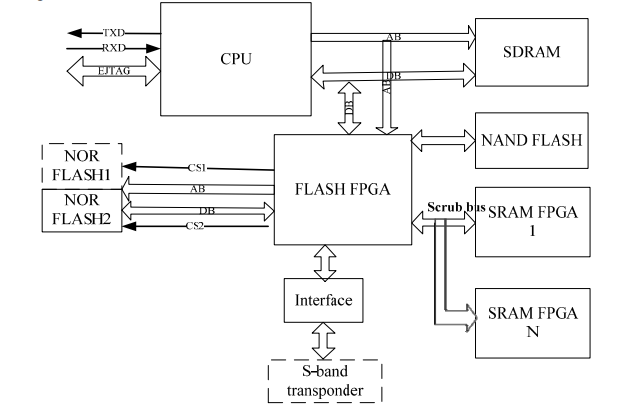
\includegraphics[scale=0.8]{images/zhou.png}
    \label{fig:zhou}
    \fonte{ZHOU et al., 2018.}
\end{figure}

Na segunda publicação estudada, o OBDH é parte de um sistema que implementa um sistema operacional em tempo real (RTOS), outro objetivo desse trabalho. Nesse caso, o OBDH é capaz de verificar telecomandos, sincronizar sistemas, reportar eventos e monitorar parâmetros (PUTRA, 2021). Seu diagrama de blocos do \textit{hardware} está disposto na Figura \ref{fig:putra}.

\begin{figure}[H]
    \centering
    \caption{Diagrama de blocos do OBDH proposto por PUTRA, 2021.}
    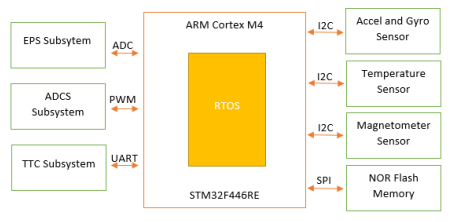
\includegraphics[scale=0.8]{images/putra.png}
    \label{fig:putra}
    \fonte{PUTRA, 2021.}
\end{figure}

No terceiro caso, a missão incluía a pesquisa e observação em órbita média (MEO), ou seja, em condições mais críticas do que o propósito do OBDH projetado nesse trabalho. Mesmo assim, as noções da arquitetura proposta são muito parecidas com o estado da arte para LEO, usando inclusive um SoC da família Zynq 7000 (LOFFLER, 2021). O diagrama de blocos do OBDH proposto nesse trabalho está disposto na Figura \ref{fig:loffler}.

\begin{figure}[H]
    \centering
    \caption{Diagrama de blocos do OBDH proposto por LOFFLER et al., 2021.}
    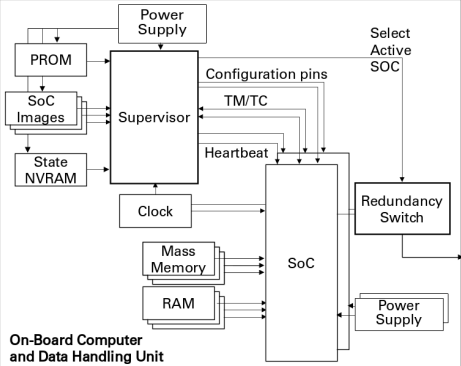
\includegraphics[scale=0.8]{images/loffler.png}
    \label{fig:loffler}
    \fonte{LOFFLER et al., 2021.}
\end{figure}

Nos três casos existem semelhanças na arquitetura, incluindo memórias usadas e interfaces de comunicação. Com isso, juntamente com o estudo dos projetos FloripaSat-1 e FloripaSat-2 e projetos comerciais, tem-se uma ampla gama de recursos a serem utilizados no critério de herança de voo para a escolha dos componentes.

\section{Metodologia para Escolha de Componentes}

Por fim, após estudar brevemente os efeitos da radiação em componentes COTS, é possível inferir uma forma de escolha dos mesmos para impactar positivamente na resistência do módulo à radiação. Por meio das diretrizes da ESA (\textit{European Space Agency}) e da NASA (\textit{National Aeronautics and Space Administration}), que já testaram componentes para os contextos de radiação em LEO, principalmente componentes passivos como capacitores e resistores, é possível fazer escolhas mais conscientes. As normas principais são a ECSS-Q-ST-60C para a ESA e da lista NPSL (\textit{NASA Part Selection List}) para a NASA.

A NPSL (Figura \ref{fig:npsl}), foi desenvolvida a fim de indicar justamente os componentes eletrônicos recomendados pela NASA. Nessa lista, se encontram componentes discretos, bem como circuitos integrados, assegurando que os mesmos foram testados em qualidade, confiabilidade e risco. 

\begin{figure}[H]
    \centering
    \caption{Interface web da NPSL.}
    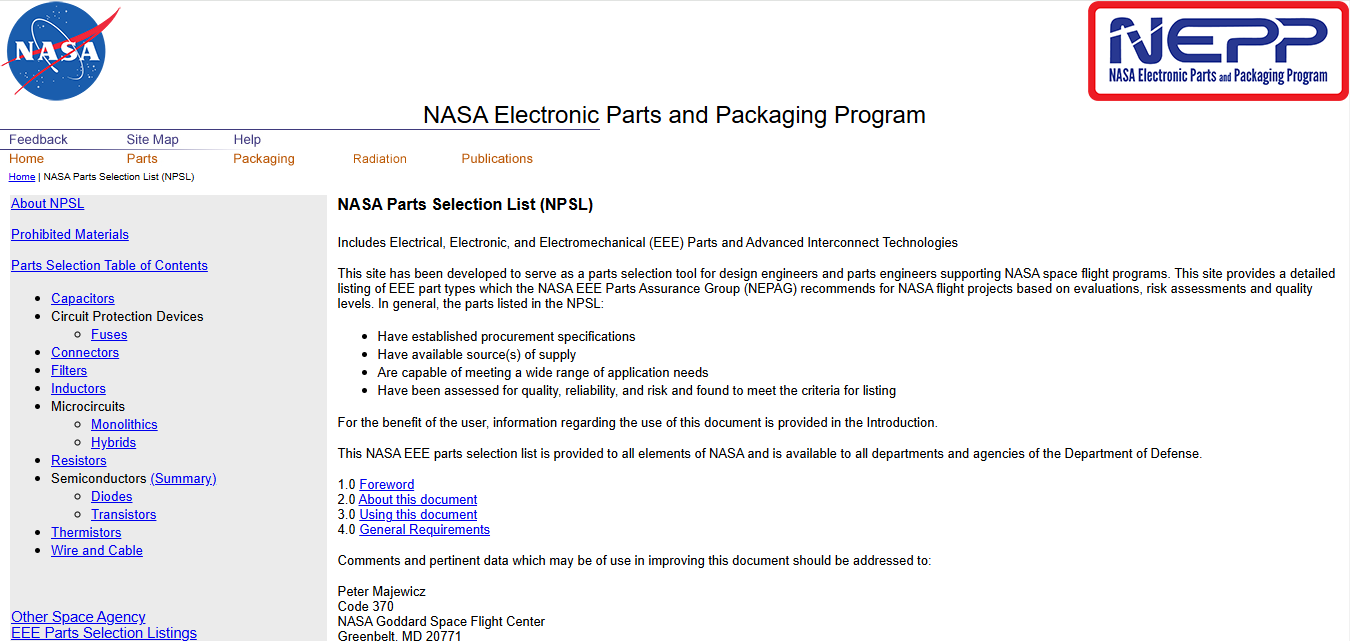
\includegraphics[width=\linewidth]{images/NPSL.png}
    \label{fig:npsl}
    \fonte{NASA, 2016.}
\end{figure}

No caso da ECSS-Q-ST-60C, há uma organização dos componentes em classes, balanceando níveis de risco e confiabilidade. Essa norma indica, de forma geral, os requisitos de seleção e uso de componentes para projetos espaciais da ESA, o que será crucial para realização desse trabalho.

Além disso, ao entender o estado da arte dos OBDHs projetados para nanossatélites, pode-se também escolher componentes por meio da herança de voo, ou seja, escolhendo componentes que já estiveram em missões semelhantes ou mais críticas.

Por fim, em alguns casos de circuitos mais complexos, os requisitos impedem que se tenha herança de voo ou que os componentes estejam presentes em uma base de dados da NASA ou da ESA. Nesse caso, será seguido cada recomendação do fabricante do circuito integrado crítico (como um SoC ou uma memória). 

Com isso, é possível começar a projetar o \textit{hardware} do OBDH, utilizando as diretrizes citadas e as heranças de voo, tomando como base os projetos citados, escolhendo os componentes e respeitando os requisitos impostos.



% Citação: 
% https://sci-hub.se/10.1109/jproc.2018.2802438
 

